\documentclass[12pt,a4paper]{article}
\usepackage[margin=1in]{geometry}
\usepackage[utf8]{inputenc}
\usepackage{amsmath}
\usepackage{amsfonts}
\usepackage{amssymb}
\usepackage{graphicx}
\usepackage{enumerate}
\usepackage{bm}
\usepackage{pythonhighlight}
\geometry{left=1.00in,right=1.00in,top=1.00in,bottom=1.00in}

\title{homework 1}
\author{Zuyao Chen 201728008629002}
\date{}
\begin{document}
\maketitle

\begin{itemize}
	\item \begin{enumerate}[(1)]
		\item  
		$p(\bm{x}|w_i)\sim N(\bm{\mu}_i,\bm{\Sigma}_i),i=1,2.$ \\ 
		we have $N = 4$ instances for both categories ,
		the mean and covariance matrix can be estimated by maximum likelihood 
		\[ \begin{split} 
		\hat{\bm{\mu}}_i &= \frac{1}{N}\sum_{n=1}^{N}\bm{x}_{i}^{(n)},i=1,2; \\
		\hat{\bm{\Sigma}}_i &= \frac{1}{N} \sum_{n=1}^{N}
						 (\bm{x}_i^{(n)} - \hat{\bm{\mu}}_i)^{T}  (\bm{x}_i^{(n)} - \hat{\bm{\mu}}_i),i=1,2
		  \end{split} 						 
		\]
		thus, 
		\[
			\hat{\bm{\mu}}_1 = (1,1)^T,
			\hat{\bm{\Sigma}}_1 =  \bm{I},
			\hat{\bm{\mu}}_2 = (5,5)^T,  
			\hat{\bm{\Sigma}}_2 = \bm{I}
		\]	
		according to the Bayesian rule,
		\[ \begin{split} 
			\text{if } &p(\bm{x}|w_1)P(w_1) > p(\bm{x}|w_2)P(w_2),\text{ then } \bm{x}\in w_1; \\
			\text{if } &p(\bm{x}|w_1)P(w_1) < p(\bm{x}|w_2)P(w_2),\text{ then } \bm{x}\in w_2 \\	
			\end{split}
		\]	
		let $f(\bm{x}) = \frac{p(\bm{x}|w_1)P(w_1)}{p(\bm{x}|w_2)P(w_2)} = 1$,
		since $P(w_1) = P(w_2) = 0.5$,
		then 
		\[
			\ln f(\bm{x}) = \ln p(\bm{x}|w_1) + \ln P(w_1) -
			  \ln p(\bm{x}|w_2) - \ln P(w_2) = 0
		\]
 		\begin{equation}
 		\label{form1}	
 			-\frac{1}{2}(\bm{x}-\hat{\mu}_1)^{T}\bm{\hat\Sigma}_1^{-1}
 		   (\bm{x}-\hat{\mu}_1) -\frac{1}{2}\ln \left|\bm{\hat\Sigma}_1\right| + \frac{1}{2}(\bm{x}-\hat{\mu}_2)^{T}\bm{\hat\Sigma}_2^{-1}
 		   (\bm{x}-\hat{\mu}_2) 
		   + \frac{1}{2}\ln \left|\bm{\hat\Sigma}_2\right|	   
 		   = 0
 		\end{equation}		
		let $\bm{x} = (x_1,x_2)^T$, formula(\ref{form1}) equals to 
		\[
		  (x_1 - 1,x_2-1)(x_1-1,x_2-1)^T - (x_1 - 5,x_2-5)(x_1-5,x_2-5)^T = 0
		\]
		\begin{equation}
			\label{form2}
			x_1 + x_2 -6 = 0
		\end{equation}
		\textbf{formula(\ref{form2}) is the equation of decision boundary}.
		\item  the graph of formula(\ref{form1}) is showed below.
		\begin{figure}[h]
			\centering
			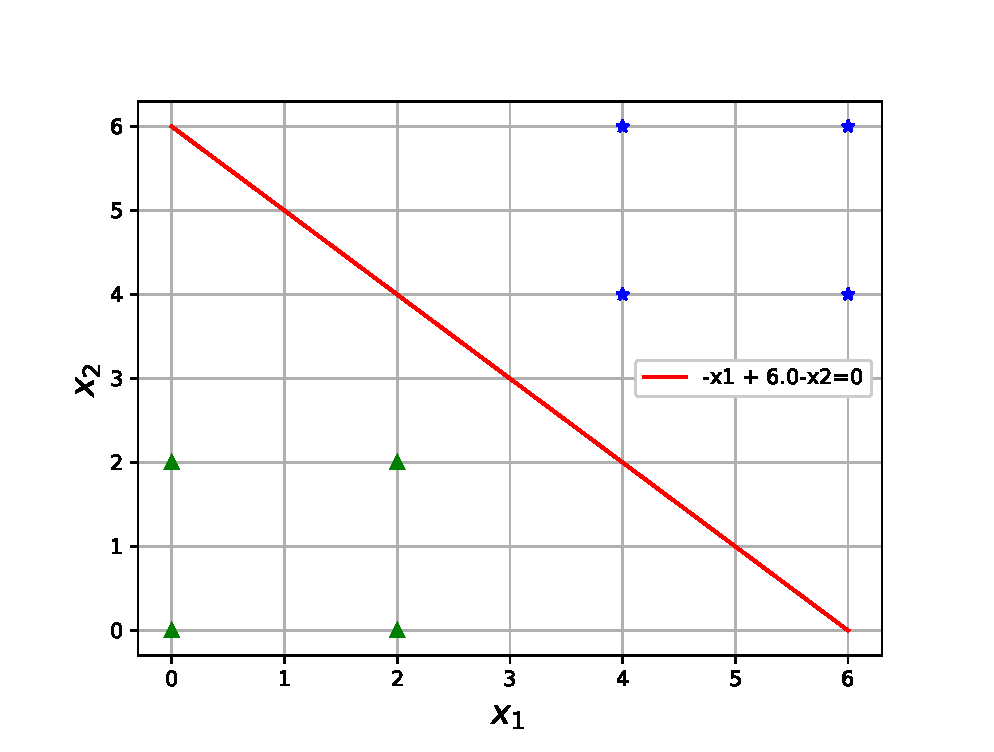
\includegraphics[width=0.6\textwidth,height=0.2\textheight]{plot1}			
		\end{figure}
	\end{enumerate} 
	\newpage
	\item the program implementation(using Python) of the question above:
	\inputpython{work.py}{1}{70}
\end{itemize}	
	

	
	
\end{document}